\chapter{Introduction}\label{sec:introduction}

Parallel and distributed computing has been utilized for decades in the high performance computing market as a means to increase performance. Parallel computing went mainstream in 2005 with the release of the first dual-core desktop processors. Almost every computer that is built today contains a multi-core processor, and many common software packages utilize parallel processing in day to day tasks. The embedded market, however, has yet to embrace parallel computing in any meaningful way. One method for utilizing parallel computing in embedded systems is to use a network of single-core embedded processors. Although the hardware already exists to implement such a network, the communications technology necessary for these processors to communicate does not yet exist. Most aspects of network communications technology are essentially solved problems, but routing has proven to be a difficult and elusive problem to solve when optimizing for distributed systems. This paper presents a prototype toolkit for embedded parallel and distributed computing that showcases a non-deterministic oblivious routing scheme that has been tailored for embedded systems.

\section{Parallel Video Transcoder - A Motivating Story}\label{sec:introduction:motivating_story}

A presentation was given at the Texas Instruments Developer Conference in 2007 titled ``A Scalable Multi-DM642-based MPEG-2 to H.264 Transcoder.'' \cite{ref:2007-raman-h.264_parallel_transcoder} The talk described a system for transcoding high definition video content encoded using the older MPEG-2 video codec to the newer H.264 video codec in real-time, a process that is too resource intensive for a single embedded processor. The system was designed to use multiple Texas Instruments DM642 Digital Signal Processors (DSPs) to cope with these requirements. 

The presenter spent much of the presentation discussing the mechanisms that were implemented to handle the communication and work sharing between DSPs. The results obtained with a two DSP system showed that they could only encode video with 75\% of the resolution of standard definition video! This equates to roughly 15\% of the resolution of a 1080p high definition video signal. Why could the end product only handle 15\% of the target goal? It can be inferred from the presentation that the developers spent much of their time setting up the basic mechanisms necessary to distribute the work load between two DSPs, instead of working on getting the algorithm to scale well to multiple DSPs. The presentation also informed the audience that the distribution mechanisms were very special-purpose, and modifying them to support more processors (or other applications) involved non-trivial modifications.

If the developers of the transcoding system had a toolkit that provided all of the basic mechanisms, including a high-performance routing algorithm, then perhaps they would have presented results showing a complete system. Such a toolkit could have also resulted in a faster time to market, and less cost in terms of engineering overhead, and one of the core components of the toolkit is the routing algorithm. It also illustrates that a complete toolkit is necessary for the development of a routing algorithm, and so a prototype toolkit is presented here that addresses the networking requirements necessary to perform routing in addition to the routing algorithm itself.

\section{Basics of Parallel and Distributed Computing}\label{sec:introduction:parallel_computing_overview}

Parallel computing is defined as dividing a program into sub-components that are executed simultaneously with the intent of decreasing execution time. Distributed computing is subtly different from parallel computing and is defined as utilizing a group of discrete processing elements to collaboratively solve a problem. A parallel computing system is often, but not always, a distributed computing system. Likewise, a distributed computing system is often, but not always, used for parallel computing. Parallel computing was initially employed in supercomputers to achieve higher performance levels. It has only been in the last few years that parallel computing has begun to appear in consumer level computers with the advent of multi-core processors. 

\subsection{Data and Processes}\label{sec:introduction:parallel_computing_overview:data_and_processes}

Computing systems can be defined using Flynn's Taxonomy, which states that all systems consist of \emph{instructions} and \emph{data} and that each can be defined as either \emph{single} or \emph{multiple}. \cite{ref:2009-barney-introduction_to_parallel_computing}

Single Instruction, Single Data (SISD) defines a serial computing system. A SISD system consists of a single processor that can only execute a single instruction at a time, and instructions can only work on a single piece of data at a time, as shown in Figure \ref{fig:introduction:sisd}.

\begin{figure}[ptb]
	\begin{centering}
		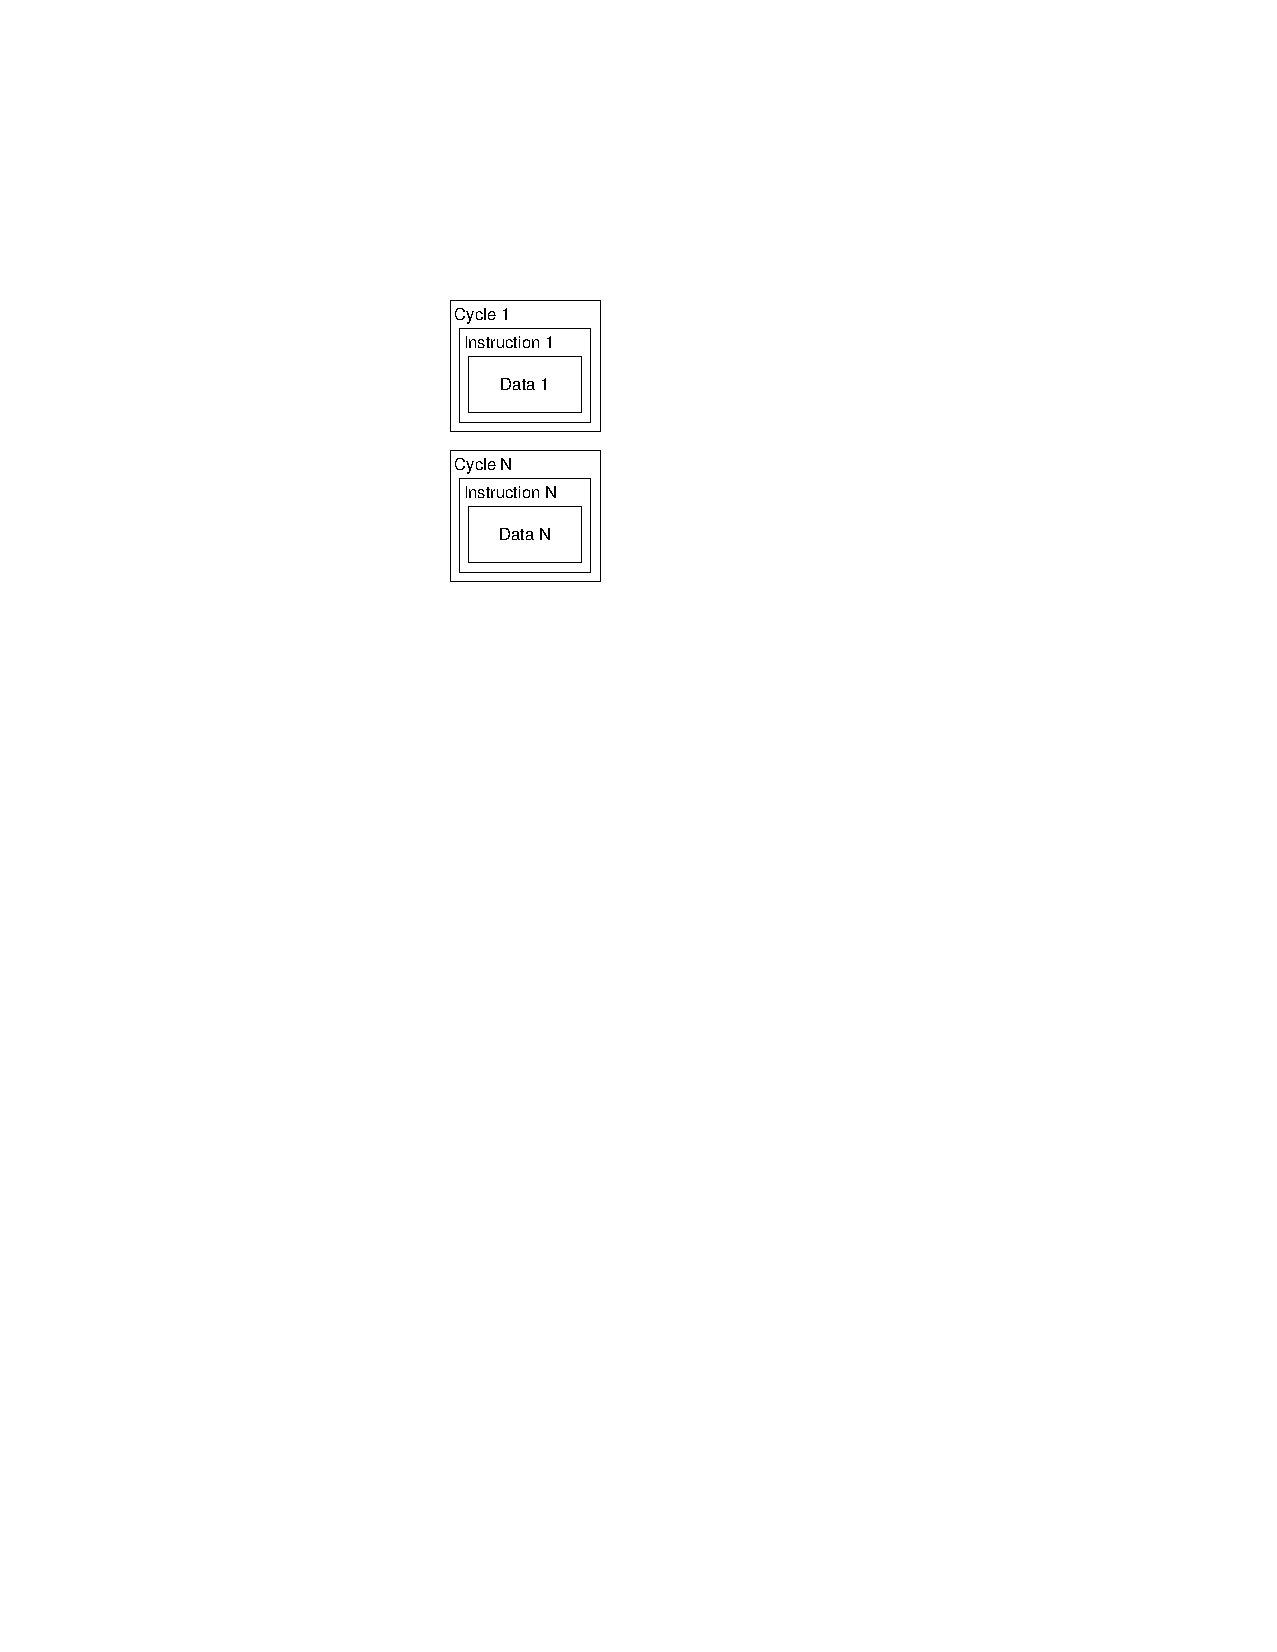
\includegraphics{Introduction/Figures/introduction-sisd.pdf}
		\caption{SISD Execution}
		\label{fig:introduction:sisd}
	\end{centering}
\end{figure}

Single Instruction, Multiple Data (SIMD) defines a computing system that executes the same instruction on several data elements at the same time, as shown in Figure \ref{fig:introduction:simd}.  This type of parallel computing is often employed when working with vectorized data, such as in image processing.

\begin{figure}[ptb]
	\begin{centering}
		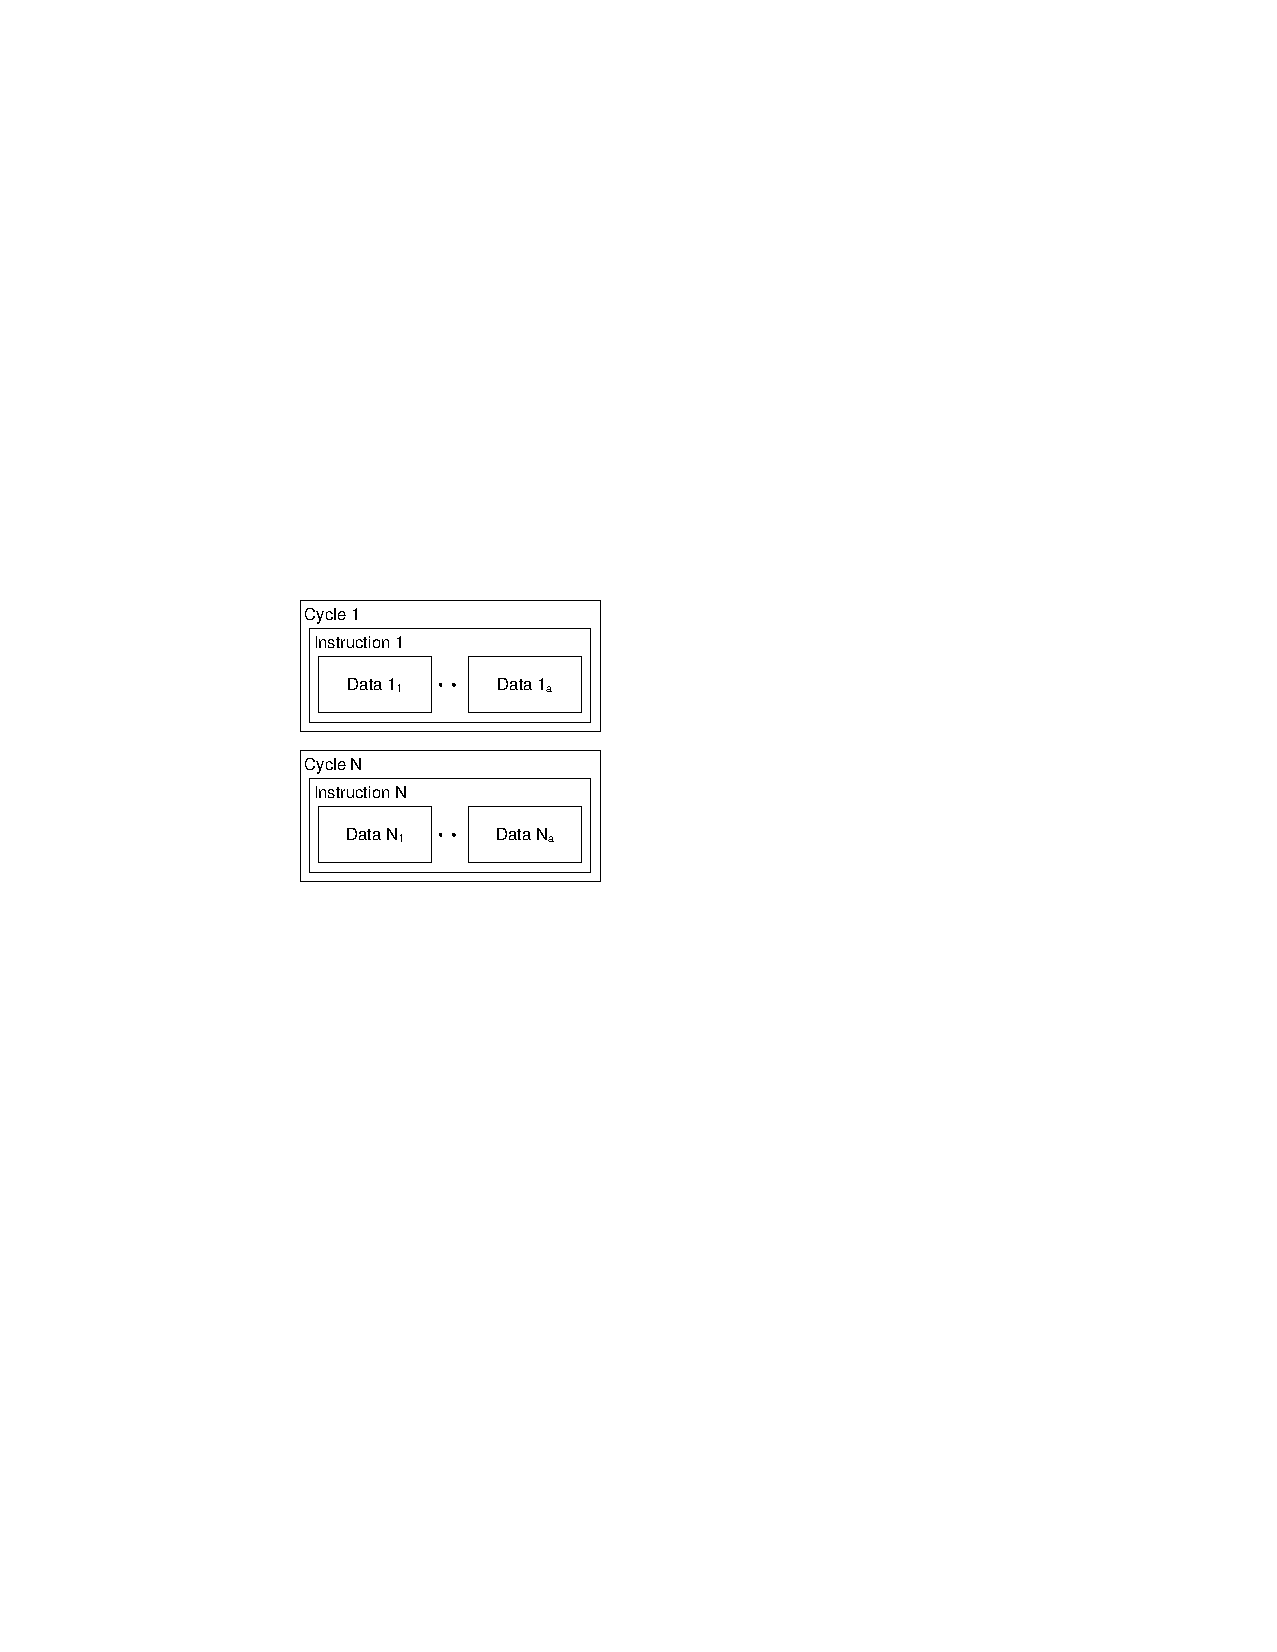
\includegraphics{Introduction/Figures/introduction-simd.pdf}
		\caption{SIMD Execution}
		\label{fig:introduction:simd}
	\end{centering}
\end{figure}

Multiple Instruction, Single Data (MISD) defines a computing system that executes multiple instructions at the same time that all work on the same data set, as shown in Figure \ref{fig:introduction:misd}. This type of parallel computing is rare but does have a few applications, such as running a single audio stream through multiple filters (e.g. an equalizer).

\begin{figure}[ptb]
	\begin{centering}
		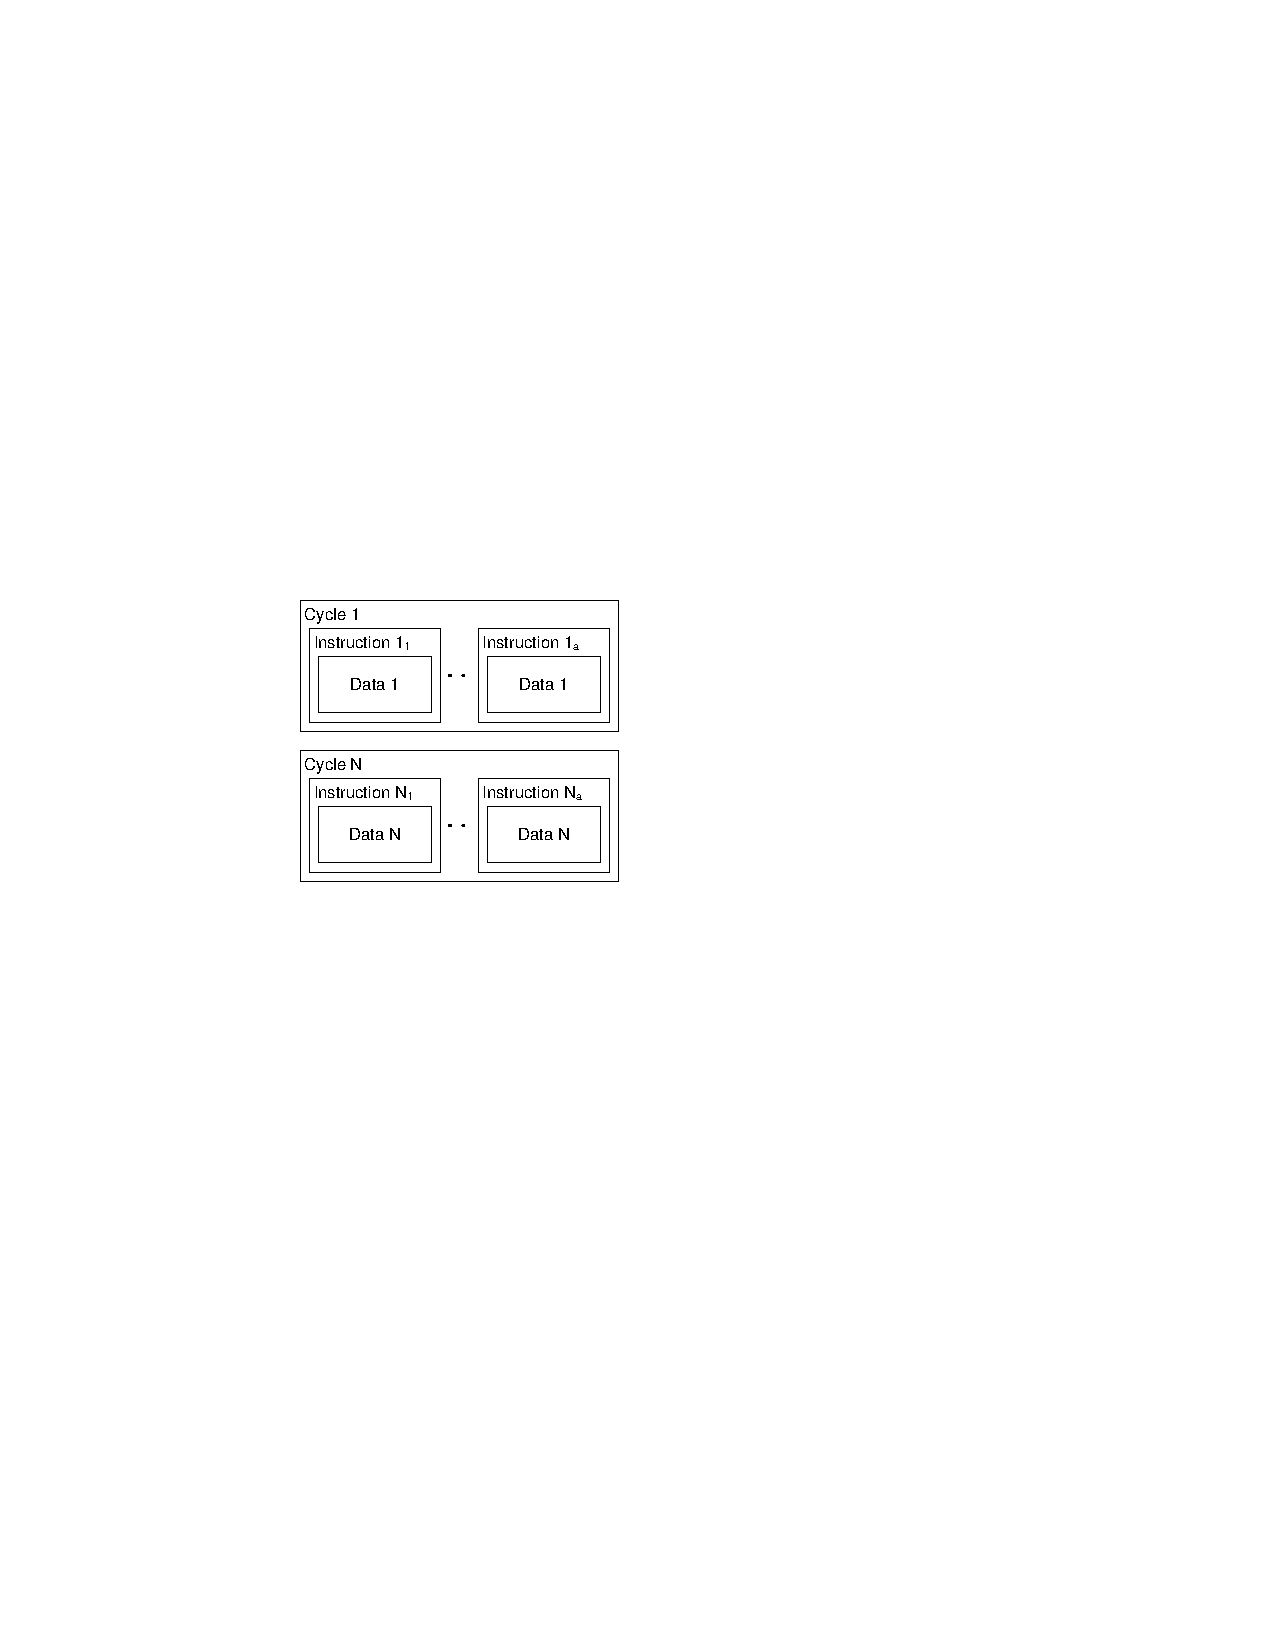
\includegraphics{Introduction/Figures/introduction-misd.pdf}
		\caption{MISD Execution}
		\label{fig:introduction:misd}
	\end{centering}
\end{figure}

Multiple Instruction, Multiple Data (MIMD) defines a computing system that executes multiple instructions at the same time that work on multiple (possibly vectorized) sets of data, as shown in Figure \ref{fig:introduction:mimd}. In practice, most modern computing systems are MIMD systems. \cite{ref:2009-barney-introduction_to_parallel_computing}

\begin{figure}[ptb]
	\begin{centering}
		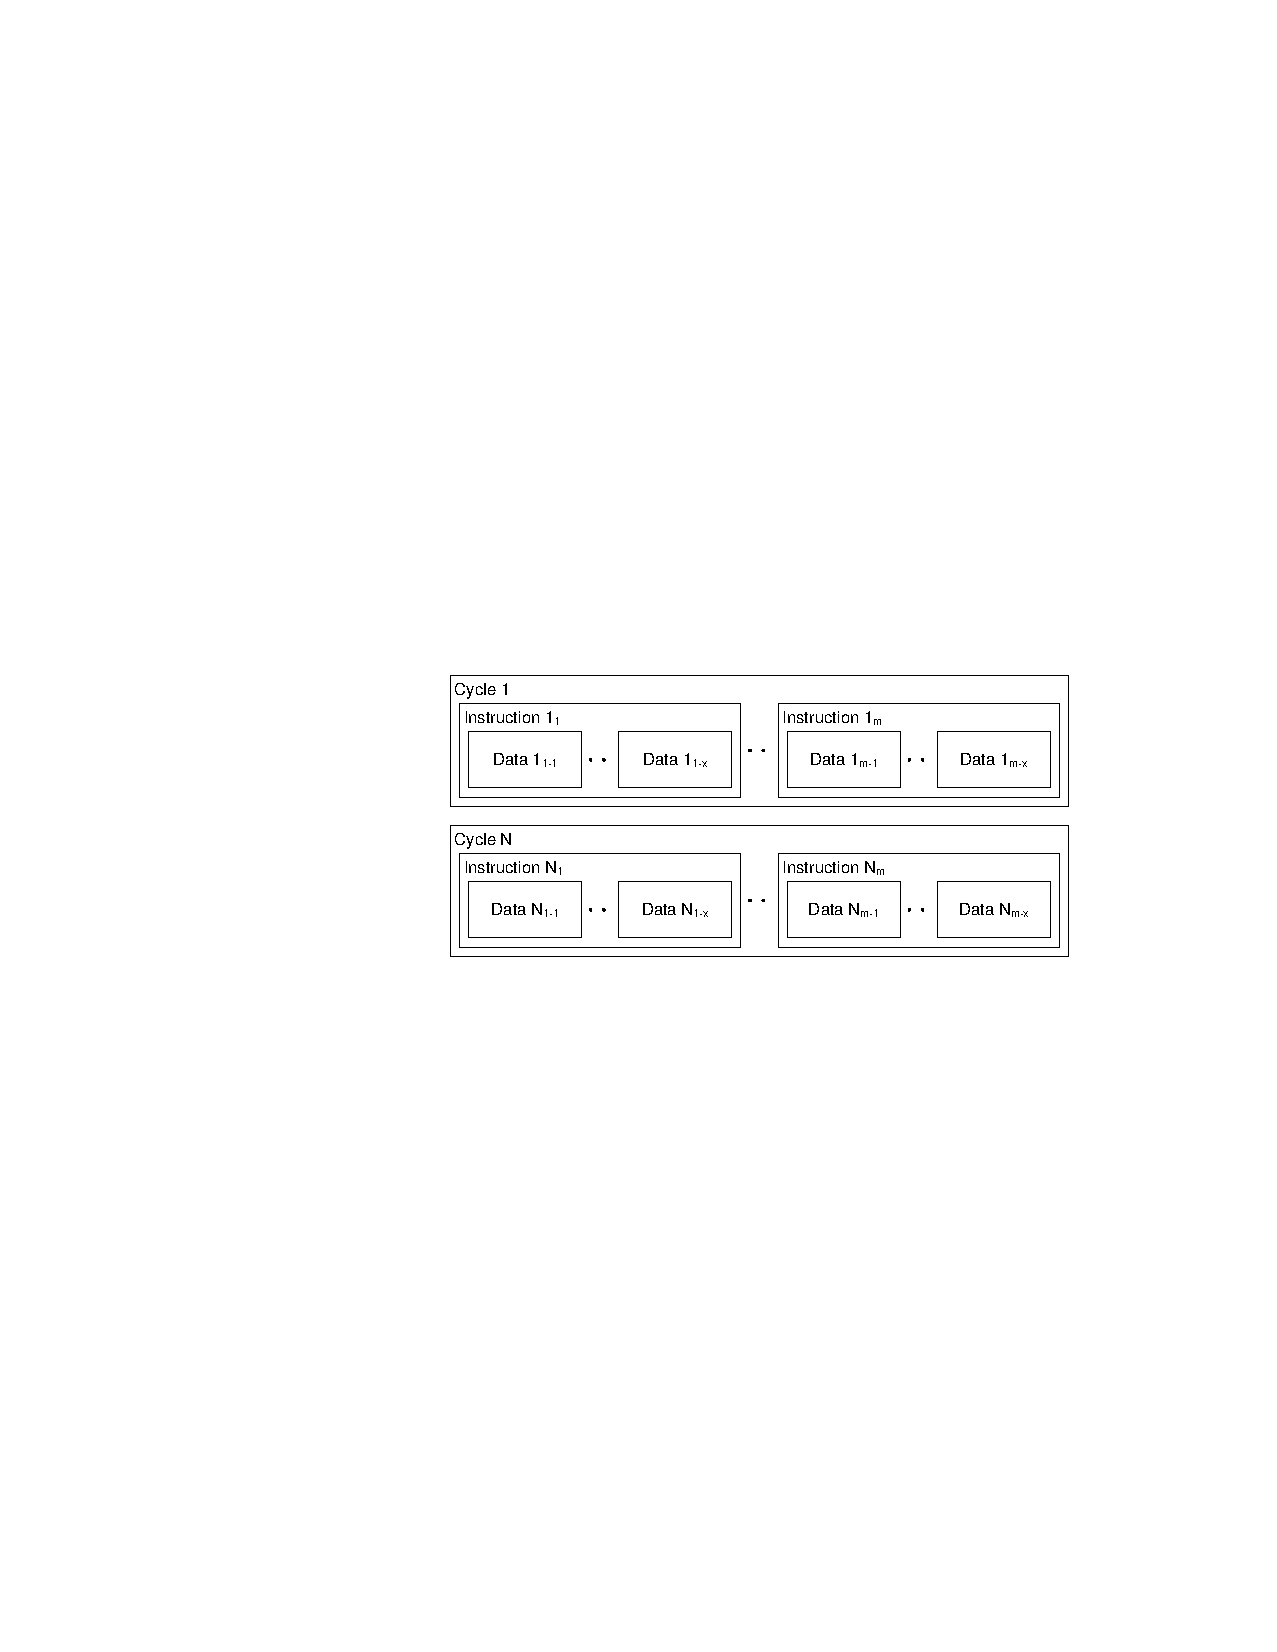
\includegraphics{Introduction/Figures/introduction-mimd.pdf}
		\caption{MIMD Execution}
		\label{fig:introduction:mimd}
	\end{centering}
\end{figure}

\subsection{Memory Architectures}\label{sec:introduction:parallel_computing_overview:memory_architectures}

In SIMD, MISD and MIMD systems, data potentially must be shared between multiple processors. The type of memory architecture employed by the system determines how data is shared between these processors. Three basic memory architectures are used in parallel and distributed systems: shared memory, distributed memory, and hybrid memory.

Shared memory systems consist of a set of processors that all have direct access to a pool of memory. Processors in a shared memory system often have hardware mechanisms to ensure cache coherency, (i.e. the local caches of each processor are kept in sync). In a Unified Memory Access (UMA) system, a single memory pool is used, as shown in Figure \ref{fig:introduction:uma}. All processors have equal access and latency to the memory. Modern multi-core consumer desktops are almost always UMA systems. In a Non-Unified Memory Access (NUMA) system, multiple memory pools are used, as shown in Figure \ref{fig:introduction:numa}. These memory pools are often associated with a specific processor, and access to this memory pool is arbitrated by said processor. This mechanism leads to an imbalance in memory latencies and access times between processors but allows greater scalability. Sometimes NUMA systems are actually distributed memory systems that utilize a software layer to make the system appear to be a shared memory system. There are also cache coherent NUMA (CC-NUMA) systems that include the previously mentioned cache coherency hardware.  Some modern workstations and almost all servers are CC-NUMA systems.

\begin{figure}[ptb]
	\begin{centering}
		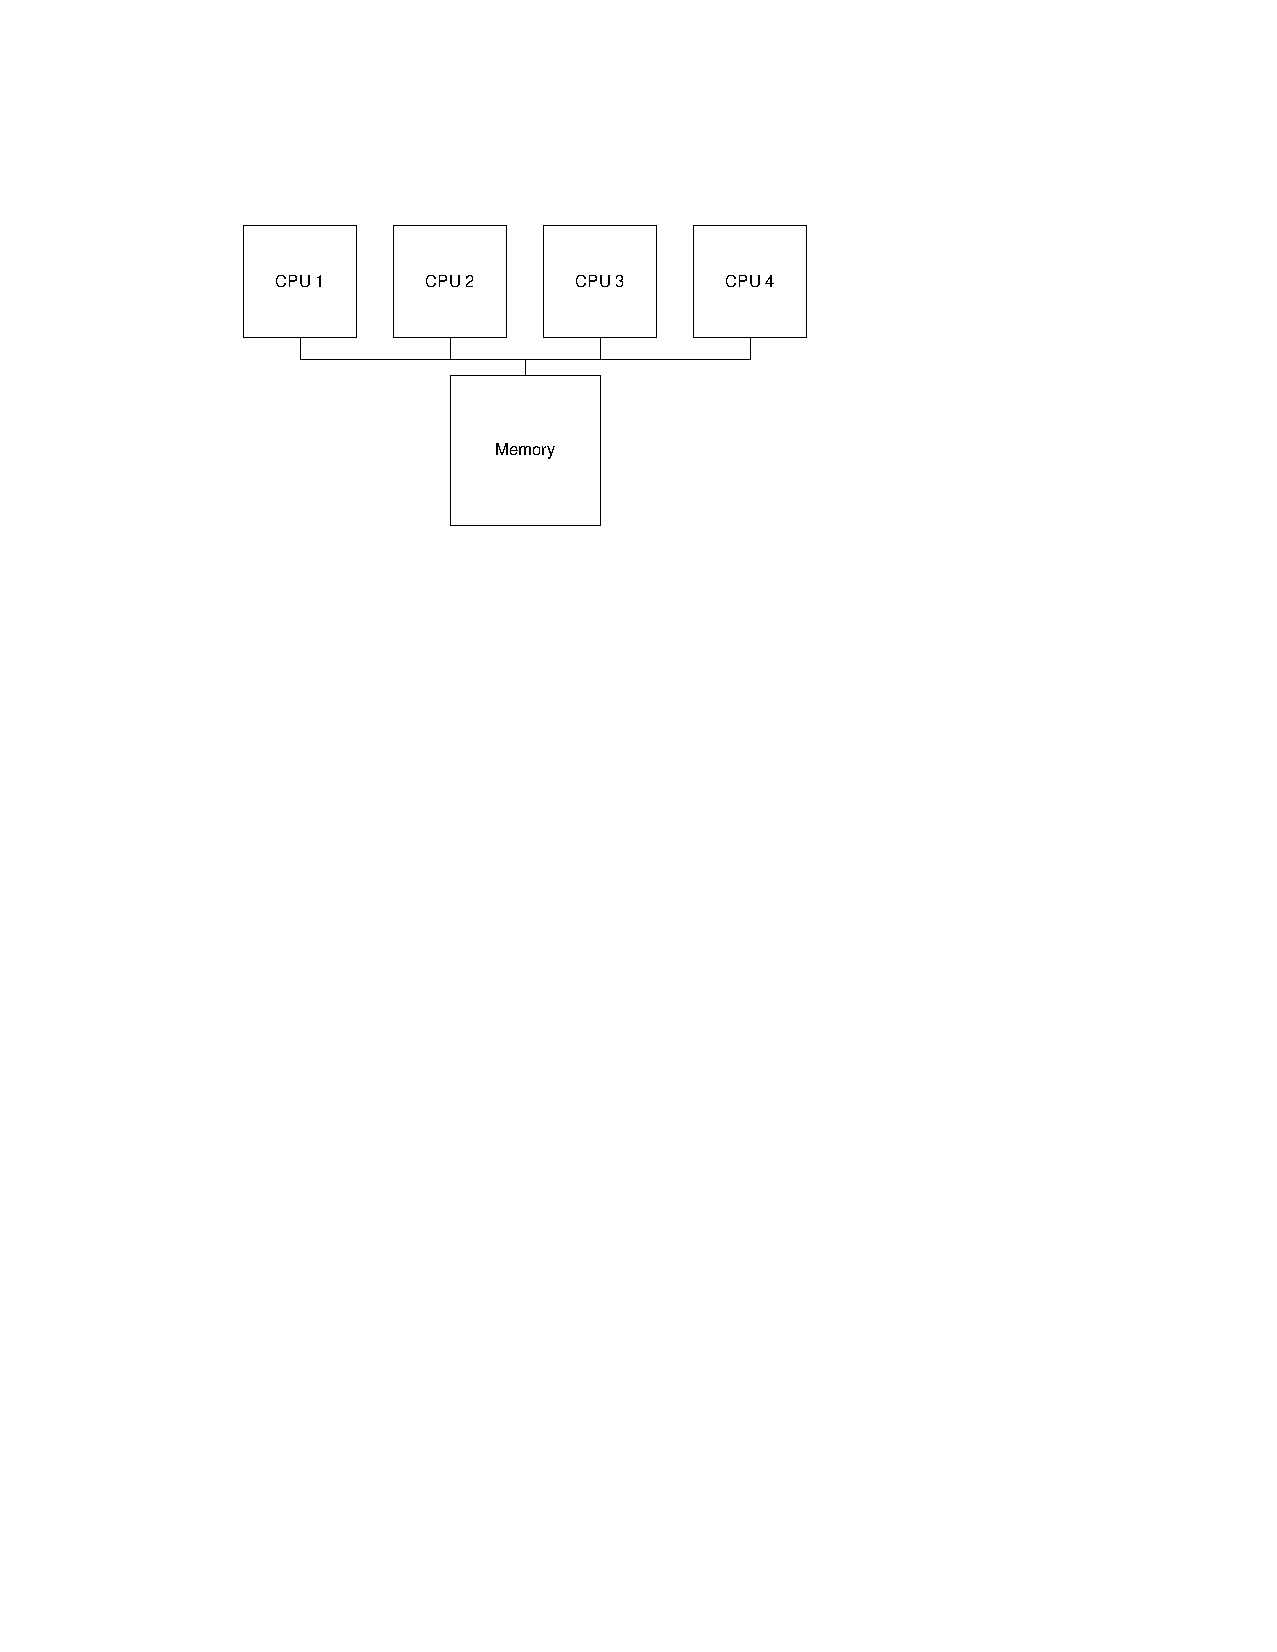
\includegraphics{Introduction/Figures/introduction-shared_memory_uma.pdf}
		\caption{Example UMA Memory Architecture}
		\label{fig:introduction:uma}
	\end{centering}
\end{figure}

\begin{figure}[ptb]
	\begin{centering}
		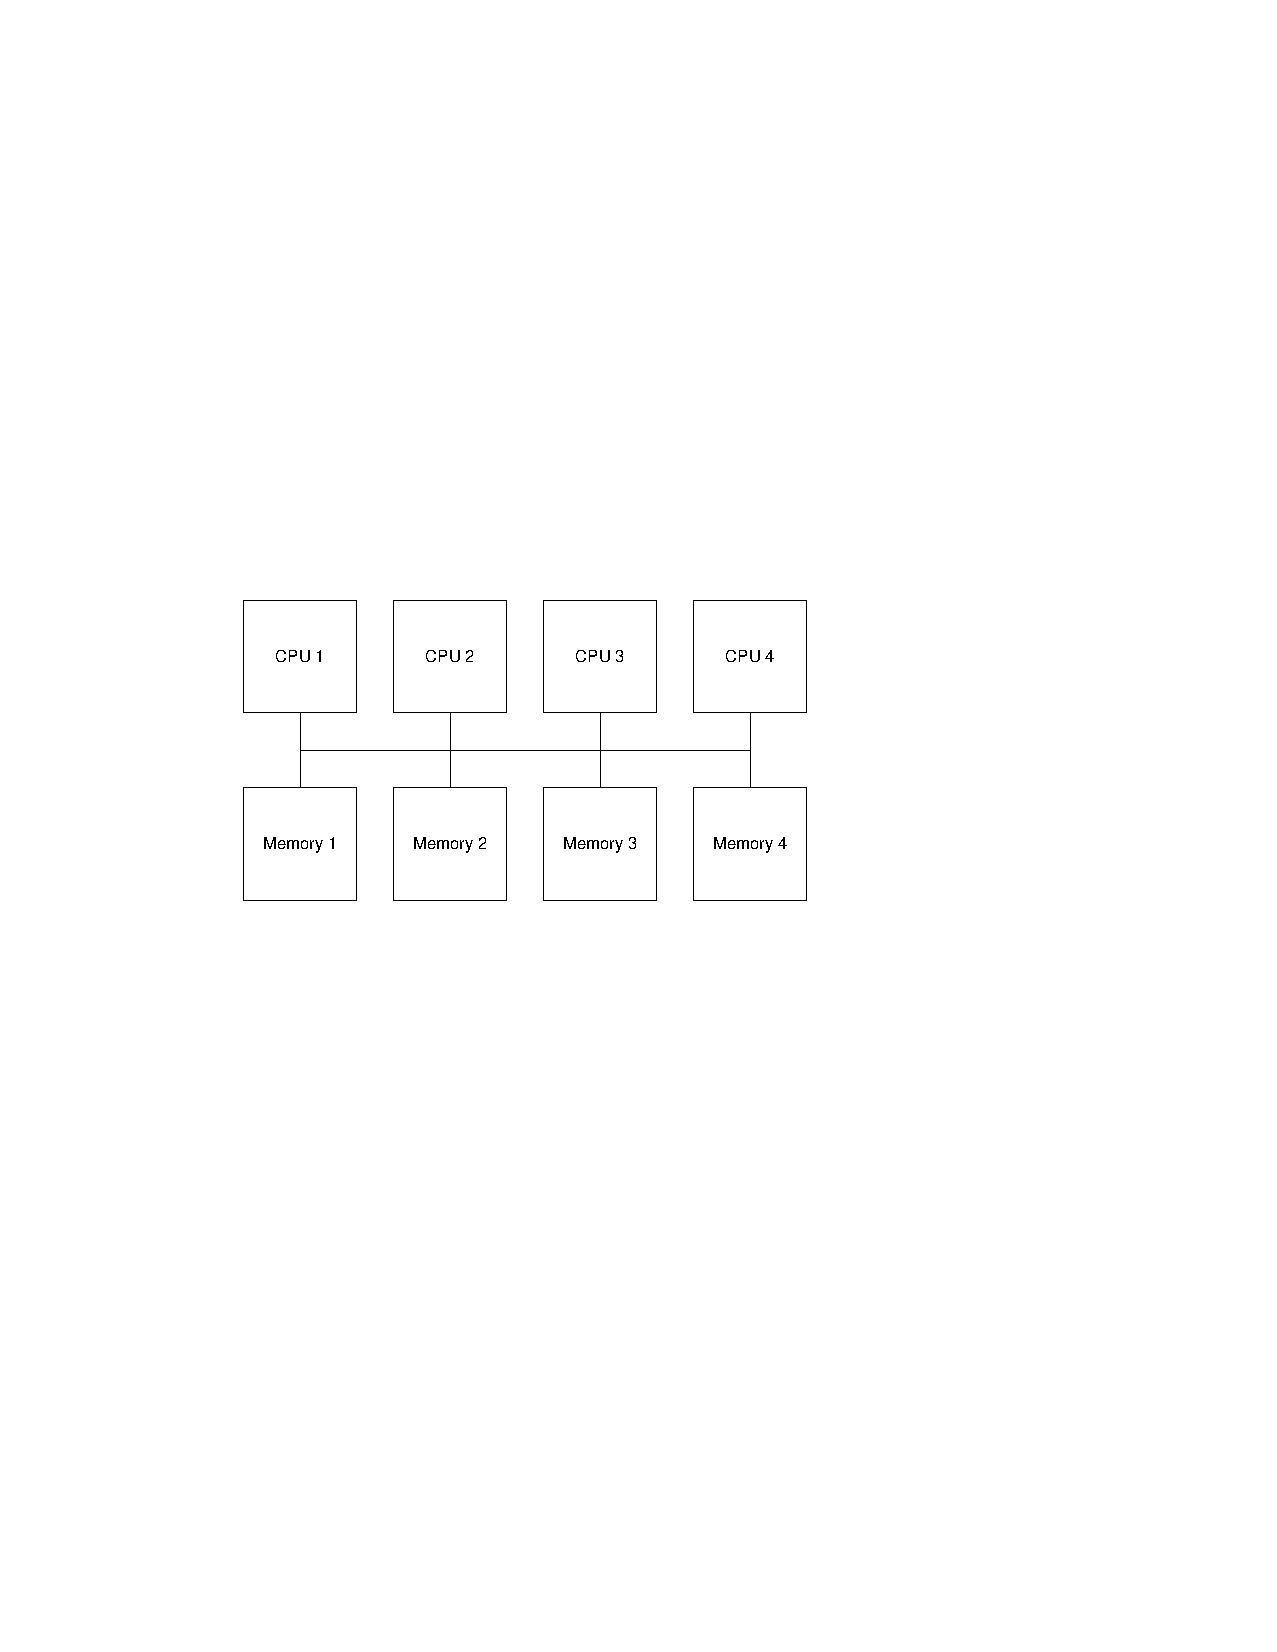
\includegraphics{Introduction/Figures/introduction-shared_memory_numa.pdf}
		\caption{Example NUMA Memory Architecture}
		\label{fig:introduction:numa}
	\end{centering}
\end{figure}

Shared memory systems are advantageous primarily because they present a unified memory pool to the programmer, which greatly reduces the programming overhead. One disadvantage is that the programmer must ensure that processors access memory ``correctly. '' For example, programmers must ensure that one processor doesn't try to write to a variable while another processor is trying to read from that same variable. Another disadvantage is that systems do not typically scale beyond 8 physical processors in practice.

In distributed memory systems, each processor typically has its own memory pool that is not globally available to other processors, as shown in Figure \ref{fig:introduction:distributed_memory}. Distributed memory systems rely on the interconnect between the processors to share data, which requires the programmer to explicitly send data from processor to processor. This increases programming compared to shared memory systems, but allows much greater scaling. Historically, many supercomputers were distributed memory systems, but they are difficult to find now due to the rise in hybrid systems.

\begin{figure}[ptb]
	\begin{centering}
		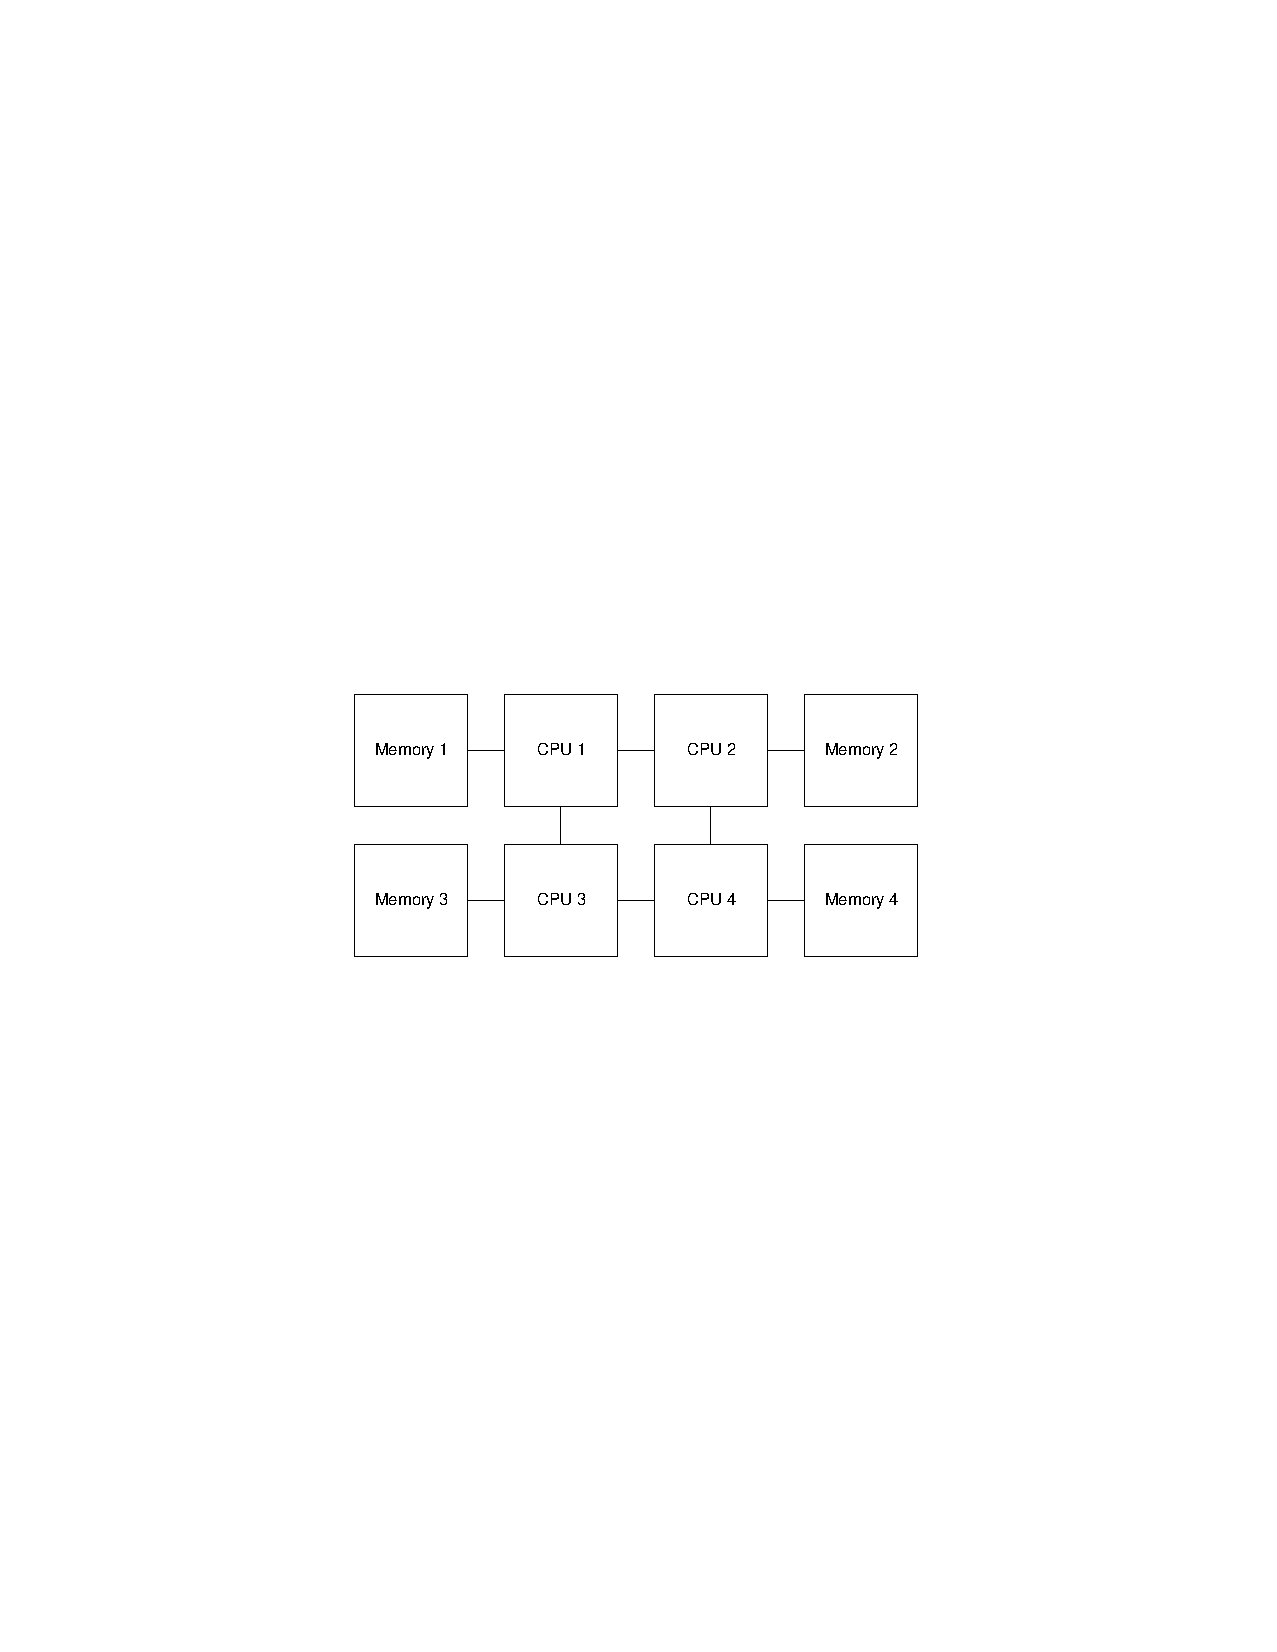
\includegraphics{Introduction/Figures/introduction-distributed_memory.pdf}
		\caption{Example Distributed Memory Architecture}
		\label{fig:introduction:distributed_memory}
	\end{centering}
\end{figure}

Hybrid memory systems consist of multiple shared memory systems connected in a distributed manner, as shown in Figure \ref{fig:introduction:hybrid_memory}. These systems commonly consist of multiple ``off-the-shelf'' UMA or NUMA computers that are connected via a networking interface such as Ethernet or Infiniband. Almost all modern supercomputers are designed this way. \cite{ref:2009-barney-introduction_to_parallel_computing}

\begin{figure}[ptb]
	\begin{centering}
		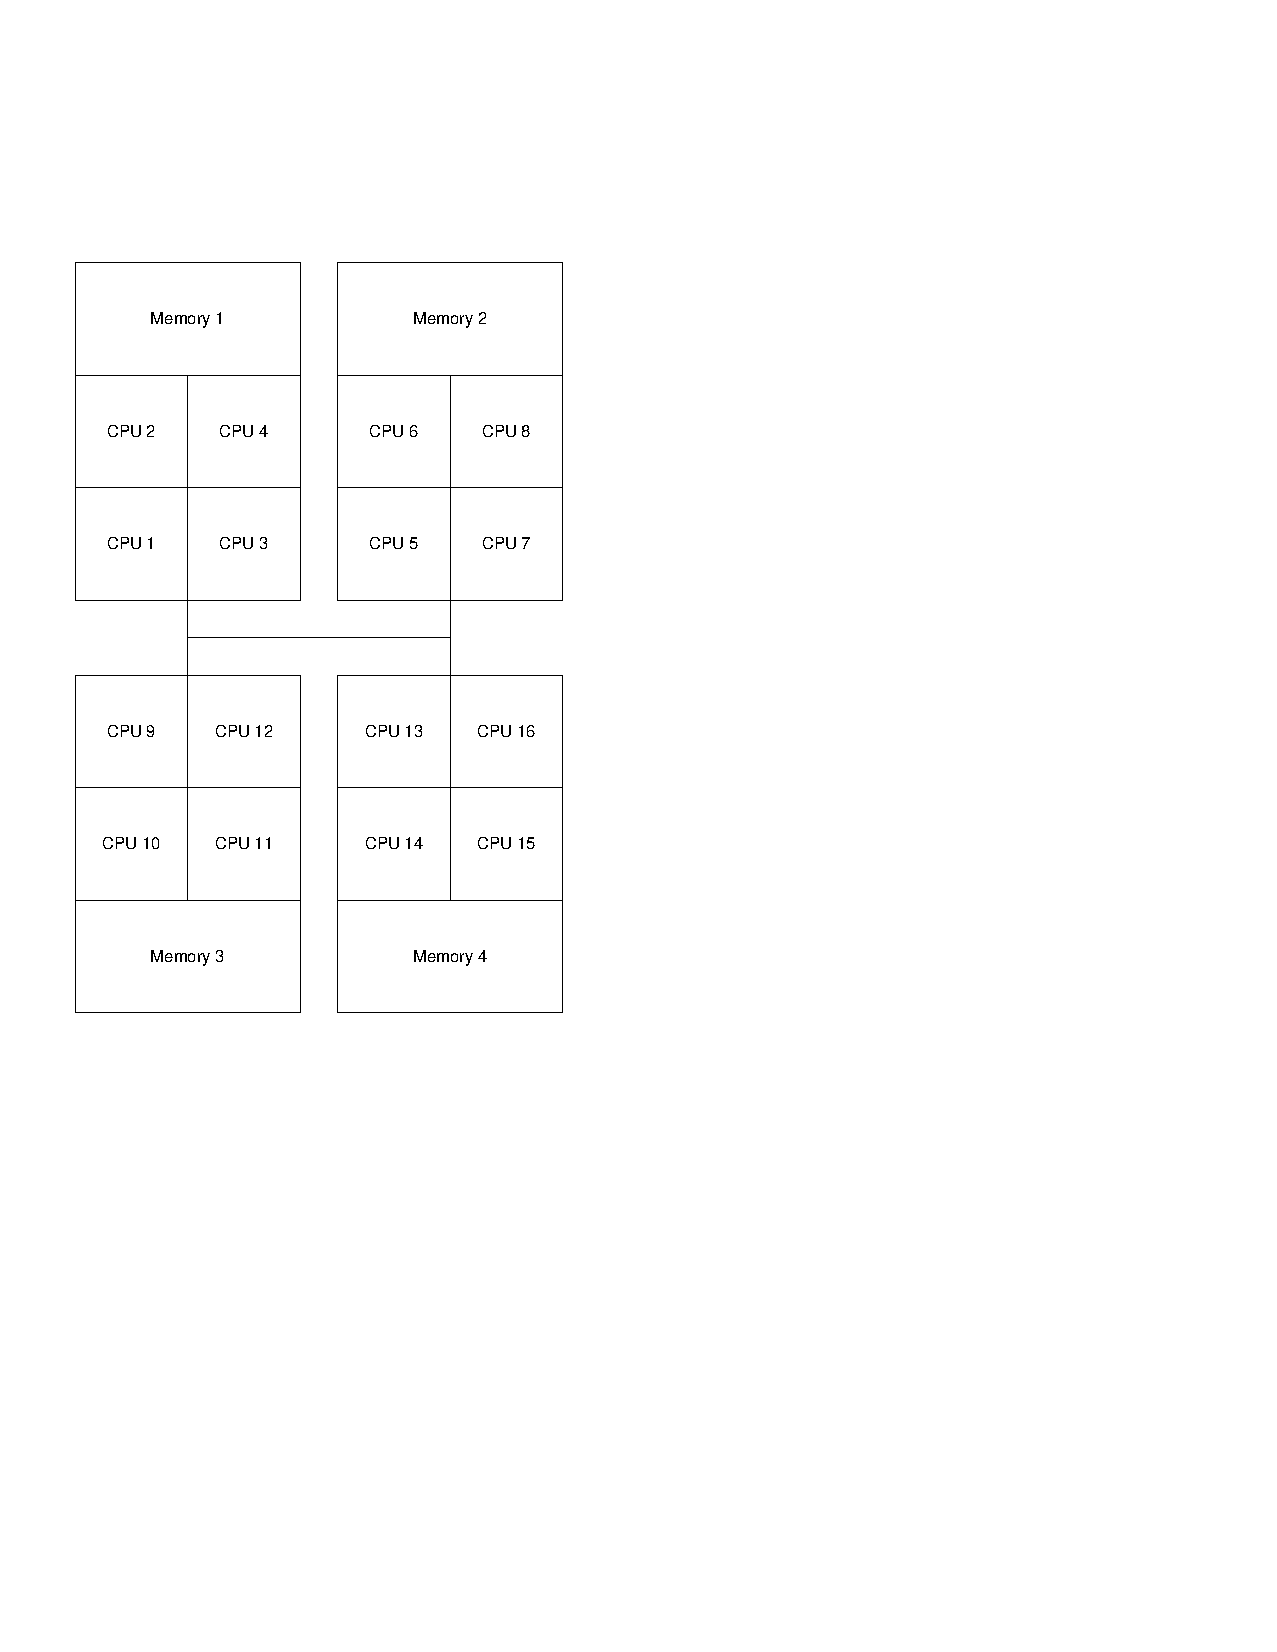
\includegraphics[height=6in]{Introduction/Figures/introduction-hybrid_memory.pdf}
		\caption{Example Hybrid Memory Architecture}
		\label{fig:introduction:hybrid_memory}
	\end{centering}
\end{figure}

\subsection{Programming Models}\label{sec:introduction:parallel_programming_overview:programming_models}

Each memory model has one or more associated programming models. Shared memory systems have several programming models that are based on the concept of threads. A thread is a block of code that is executed independently of other threads. Each thread has its own stack and local variables that are independent of other threads, but everything else is shared. Data that is accessed by multiple threads is declared global because global memory is shared among threads. Locking mechanisms, such as semaphores, are employed to ensure correct access. Threads do not need to execute the same code and can also be used for purposes other than parallel computing. This model results in greater flexibility at the expense of greater complexity. Several higher-level models have been developed explicitly for parallel computing that use threads under the hood. The most prominent model is OpenMP, which uses code markup to signify where to parallelize code.

Distributed memory systems typically use a message passing model. In the message passing model, a node will send a message containing the data required for execution to another node. This type of system usually employs a ``master'' or ``root'' node that manages data handling between nodes. Examples of message passing systems include the Message Passing Interface (MPI) and the Parallel Vector Machine (PVM) Application Programming Interfaces (APIs). MPI can also be used on shared memory systems, but usually isn't due to a performance disadvantage compared to threading models. Hybrid systems can use a combination of the shared memory models and message passing models. \cite{ref:2009-barney-introduction_to_parallel_computing}

Systems do exist that aren't quite shared memory systems, but aren't quite distributed memory systems either, in the classical sense. The video transcoder example is one of these and is essentially a NUMA shared memory system, but requires explicit synchronization by the programmer. Data transfers are handled by Direct Memory Access (DMA), which imposes extra requirements on how data is handled and processed, thus increasing complexity. 

\section{Motivation}\label{sec:introduction:motivation}

1 
Distributed computing has been used in embedded systems for a long time, but in a manner different than standard computing systems. Embedded distributed computing was first used on a large scale in automotive systems, where sensing systems were separated by physical distance. These systems typically involved a sensor that contained processing logic used to communicate with a master processor. The distributed sensors were not used for processing; thus these systems were not parallel computing systems. As a result, the distributed computing mechanisms evolved differently than their computer brethren.

The recent emergence of high definition (HD) media and interactive portable devices, such as smartphones, GPS units, and media players, has caused a shift in the embedded market towards higher performance. In some cases these new technologies have also created a market for higher-end equipment in the associated infrastructure that uses embedded processors. In fact, data traffic in cellular networks has been growing exponentially since 2001 \cite{ref:2008-ohult-the_mobile_broadband_evolution}.

Parallel computing is beginning to show up in high-end embedded systems, especially in commercial wireless communications systems. Many modern cellular baseband processing systems are comprised of multiple DSPs and a Field Programmable Gate Array (FPGA) device. Example systems are described in \cite{ref:2007-wilson-using_serial_rapidio_switches} where multiple DSPs and an FPGA are used as the software-defined-radio component of the baseband processing system.

The hardware resources available for parallel computing at the high-end are very compelling, but they are currently high-end only; there are no multi-core mainstream processors, and interconnection systems designed for parallel computing, such as RapidIO, are also high-end only. In addition, the only standardized programming models in existence are a few experimental MPI implementations, none of which are ready for commercial deployment. Routing algorithms used in embedded networks are typically very basic (such as Dijkstra's algorithm \cite{ref:2006-black-dijkstras_algorithm}), and there exists an opportunity for a high-performance routing algorithm to improve the overall performance of these systems. Embedded systems require a routing algorithm that is well suited to the limited resources available, and traditional high-performance routing algorithms are not resource friendly. A new routing algorithm is required that reduces congestion and is fault tolerant while requiring few computational or memory resources.

\section{Objectives}\label{sec:introduction:objectives}

The purpose of the research presented here is to provide a toolkit containing mechanisms necessary to develop distributed and parallel applications for mainstream embedded hardware in an efficient manner. The toolkit must be sufficiently easy to use that an overall net gain in productivity is seen on the part of the application engineer. This ease of use can be achieved by providing simple and automated network configuration and by using established programming models.

The toolkit proposed here targets mainstream processors and their capabilities. The toolkit will be a distributed memory system and will use message passing to share data because shared memory would require specialized hardware. The toolkit is divided into the following parts:

\begin{itemize}
	\item Physical and Data Link Layer Communications
	\item Network Layer Protocol
	\item Routing in Embedded Systems
	\item MPI Application Layer
\end{itemize}

The physical and data link layer, discussed in Chapter \ref{sec:spi}, is responsible for managing the hardware communications interface and low level protocol used for communicating between direct neighbors, and must meet the following criteria: links must be self-configuring, links must be scalable, the communications interface selected must be available on a wide variety of devices, and the communications interface must be point-to-point. The criteria for the four parts will be discussed in further detail in the later sections.

The network layer protocol, discussed in Chapter \ref{sec:protocol}, is responsible for handling communications between a given source and destination, and all activities related to these communications. The protocol must meet the following criteria: it must support ``end-to-end'' transmissions, provide dynamic and self-configuring addressing, provide error checking, be of a proper complexity for mainstream embedded systems, and be fault tolerant.

The routing scheme, discussed in Chapter \ref{sec:routing}, determines how traffic is routed through the network and must meet the following criteria: it must be self-configuring, it must be applicable to general networks, it must utilize communication resources efficiently, and it must use processing resources efficiently.

MPI, discussed in Chapter \ref{sec:api}, is implemented in the application layer to provide a framework that existing parallel programmers will recognize. It must meet the following criteria: it must implement a subset of the MPI 1.1 specification, all methods that are implemented must be compatible with the existing specification, and it must not require any configuration outside of normal MPI configuration.

The toolkit is considered complete when all of the aforementioned criteria are met. In addition to these four parts, this paper also discusses prototype circuit boards that contain an F2808 Digital Signal Controller (DSC) for testing and profiling the toolkit software in Chapter \ref{sec:hardware}.